% =========================================================================
% Metaheuristics Project (31-MM34, SoSe 26) -- Full Report (V2)
% Structure identical to Report_Structure_V2.tex.
% Compile: pdflatex Report_Full_V2.tex  (convergence.png must be present)
% =========================================================================
\documentclass[10pt, a4paper]{article}

\usepackage[utf8]{inputenc}
\usepackage[T1]{fontenc}
\usepackage{lmodern}
\usepackage[margin=2.5cm]{geometry}
\usepackage{amsmath,amssymb}
\usepackage{booktabs}
\usepackage{graphicx}
\usepackage[hidelinks]{hyperref}

\title{An Adaptive Large Neighborhood Search for the\\
       Prize-Collecting Skill Vehicle Routing Problem}
\author{Umais Chaudhary, Rehman Kerimov, Dustin Schulz, Marco Leander vom Orde \\
        \small 31-MM34 Metaheuristics, SoSe 26, Bielefeld University}
\date{July 2026}

\begin{document}
\maketitle

% -------------------------------------------------------------------------
\section{Introduction}

A pharmacy delivers medication to patients at home. Each delivery may require
a qualification (administering an injection, handling refrigerated goods),
each courier holds a subset of these skills, and not every patient can be
served within the couriers' shifts. The dispatcher therefore faces a
\emph{prize-collecting} problem: select which customers to serve at all, and
route the couriers so that the collected profit is maximized.

Formally, an instance consists of customers $C=\{1,\dots,n\}$ with profit
$p_i$, service time $s_i$, time window $[r_i, d_i]$ and required skill set
$Q_i$, and couriers $B=\{1,\dots,b\}$ with skill set $S_k$ and shift
$[a_k, e_k]$. All tours start and end at the pharmacy (node~0), and travel times
are Euclidean distances rounded down. Courier $k$ may serve customer $i$ only
if $Q_i \subseteq S_k$. Service must start within $[r_i,d_i]$ (early arrival
waits), and the courier must return to the depot by $e_k$. Each customer is
served at most once, and unserved customers simply yield no profit. The objective
is to maximize $\sum_{i \in C'} p_i$ over the set $C'$ of served customers.
The empty plan is always feasible, so the problem is one of profitable
selection rather than mere feasibility.

As a yardstick we use the \emph{singleton upper bound}
$\mathrm{UB} = \sum_i p_i \cdot [\,\exists k: \text{$i$ alone is feasible for
$k$}\,]$: the profit of all customers that at least one courier could serve
in a dedicated round trip. UB ignores that customers compete for shift time,
so it is loose, particularly when few couriers share many reachable
customers, but it is cheap, instance-independent and allows relative
comparisons across instance sizes.

The report follows our development path: the literature fixes the method
family (Section~2), a simple construction heuristic fixes the baseline
(Section~3.1), and engineering makes move evaluation cheap enough for pure
Python under a wall-clock budget (Section~3.5). Operator breadth is then
added and
\emph{measured} rather than argued, by a leave-one-out ablation and a
parameter study (Section~4). Section~5 reports the resulting performance
under the official 30\,s budget and in 10-minute runs.

% -------------------------------------------------------------------------
\section{Choice of Method}
\subsection{Related Work}

Selecting profitable customers under routing constraints is the
\emph{orienteering} / \emph{prize-collecting} family: the team orienteering
problem with time windows (TOPTW) is our problem without skills and shifts.
Surveys by Vansteenwegen et al.~\cite{vansteenwegen2011} and Gunawan et
al.~\cite{gunawan2016} show that the strongest TOPTW heuristics are
insertion-based local search and large neighborhood schemes, e.g.\ the LNS of
Labadie et al.~\cite{labadie2012} and the iterated approach of Hu and
Lim~\cite{hulim2014}. Skill compatibility is studied as the Skill VRP by
Cappanera et al.~\cite{cappanera2011} and, closest to our setting, in
service-technician routing by Kovacs et al.~\cite{kovacs2012}, who solve a
prize-collecting routing problem with qualifications and time windows using
adaptive large neighborhood search (ALNS). Home health care routing shares
the same structure~\cite{cisse2017}. ALNS itself goes back to Shaw's
relatedness-based removal~\cite{shaw1998} and was formalized with adaptive
operator weights and simulated-annealing acceptance by Ropke and
Pisinger~\cite{ropke2006,pisinger2007}. Insertion feasibility in constant
time via forward time slacks is due to Savelsbergh~\cite{savelsbergh1992}.
More recent LNS variants contribute additional operators: sequence- and
saving-based removals~\cite{hammami2020}, time-oriented relatedness
\cite{demir2012}, and slack-induced string removals~\cite{christiaens2020}.

\subsection{ALNS justification}

Three properties of the problem drove the choice. First, the search must
jointly decide \emph{selection} and \emph{routing}: destroy/repair moves
manipulate the served set directly (a repair step may insert previously
unserved customers), whereas classical edge-exchange neighborhoods keep the
customer set fixed and would need a separate selection mechanism. Second,
the benchmark is extremely heterogeneous ($n=50$ to $1000$, 2 to 25
couriers, skill scarcity $k=0$ to $2$): with a fixed 30\,s budget in pure
Python our iteration throughput spans two orders of magnitude ($\sim$30{,}000
iterations on $n{=}50$, $\sim$600 on $n{=}1000$). An \emph{adaptive} scheme
that reweights operators online by their measured usefulness \emph{and cost}
transfers across this range without per-instance tuning. Third, skills and
tight windows make feasibility rugged, and simulated-annealing acceptance over a
penalized objective lets the search cross infeasible ridges. ALNS combines
all three ingredients in one well-understood framework~\cite{ropke2006} and
was validated on the closest published relative of our
problem~\cite{kovacs2012}.

% -------------------------------------------------------------------------
\section{Approach Description}
\subsection{Initial Greedy solution}

The construction heuristic sorts all customers that at least one courier
could serve alone by \emph{decreasing profit} and inserts each at the
cheapest feasible position (minimal travel-time increase) over all
skill-compatible couriers, and customers without a feasible position are left
unserved (pseudocode in the Appendix). The skill prefilter (per-customer
list of compatible couriers) is
precomputed once. Construction takes $<0.5$\,s even for $n=1000$ and reaches
on average 46.4\,\% of UB (range 40.5--52.6\,\%) over the 20 benchmark
instances.

To validate the profit ordering we compared against random insertion orders
(same cheapest-insertion machinery, 5 seeds): random construction reaches
only $68.6\,\%$ of the greedy profit on average (e.g.\ $n{=}1000$:
$18{,}648 \pm 831$ vs.\ $27{,}323$), with the gap widening on larger
instances. Profit ordering is essentially free and supplies about two thirds
of the final solution quality (cf.\ Table~\ref{tab:results}). We also tried
a multi-start variant over four orderings (profit, profit density, fewest
compatible couriers, hybrid). It improves the \emph{start} by up to 10\,\%,
but it also quadruples construction time, time deducted from the ALNS
budget, and it had no measurable effect on the \emph{final} result: the
ALNS absorbs start-quality differences of this size within seconds
(Fig.~\ref{fig:convergence}), faster than the extra constructions pay off.
The submitted solver therefore keeps the single profit ordering.

The construction also carries the feasibility guarantee of the whole solver:
customers are only ever placed at positions where time windows, shift and
skill constraints hold, so the start solution is feasible by design. In the
degenerate case that no customer fits anywhere, the result is the empty
plan, which is always feasible. Hence the solver can output a valid solution
for any instance and any time limit.

\subsection{ALNS Framework}

Algorithm~\ref{alg:alns} shows the main loop, where $x$ denotes the current
solution and $x^{*}$ the best feasible solution found so far. Per iteration
one destroy and one compatible repair operator are drawn by roulette-wheel
selection over adaptive weights, applied to the current solution, and the
result is accepted by simulated annealing on a penalized score. Weights are
updated segment-wise. After 500 consecutive rejections the search concludes
that it is trapped in a local optimum too deep for the destroy steps to
escape (near the end of the cooling curve even large removals are rarely
accepted) and, since budget remains, forces the exit: $x$ is replaced by a
fresh randomized greedy solution (random insertion order, cheapest feasible
positions) and the temperature is reheated to $0.75\,T_0$, giving the
remaining time a second, slightly cooler annealing pass.

\begin{figure}[t]
\small
\hrule\vspace{2pt}
\textbf{Algorithm 1:} ALNS for the prize-collecting Skill VRP
\vspace{2pt}\hrule\vspace{4pt}
\begin{tabbing}
\hspace{1.2em}\=\hspace{1.2em}\=\hspace{1.2em}\=\kill
$x \leftarrow$ greedy construction; \quad $x^{*} \leftarrow x$; \quad
$T \leftarrow T_0$\\
\textbf{while} wall-clock time remains \textbf{do}\\
\>choose destroy $d$ and repair $r$ by roulette wheel over weights $w$\\
\>$x' \leftarrow r(d(x))$
  \quad\emph{(remove $q$ customers, reinsert removed + sampled unserved)}\\
\>\textbf{if} $\exp\bigl((f(x') - f(x))/T\bigr) > u \sim U(0,1)$
  \textbf{then} $x \leftarrow x'$
  \quad\emph{(penalized score $f$)}\\
\>\textbf{if} $x'$ feasible \textbf{and} $\mathrm{profit}(x') >
  \mathrm{profit}(x^{*})$ \textbf{then} $x^{*} \leftarrow x'$\\
\>credit $d$ and $r$ with score $\sigma \in \{25, 10, 3, 0\}$; record their runtime\\
\>\textbf{every} $L$ iterations: \(w \leftarrow (1-\rho)\,w +
  \rho\,\dfrac{\bar\sigma}{1 + (\bar t / \tau)^{\alpha}}\)
  \quad\emph{(runtime-normalized utility)}\\
\>update $T$ on the exponential wall-clock schedule $T_0 \to T_{\min}$\\
\>\textbf{if} 500 consecutive rejections \textbf{then} $x \leftarrow$
  randomized greedy; \ $T \leftarrow \max(T,\, 0.75\,T_0)$
  \quad\emph{(restart + reheat)}\\
\textbf{return} $x^{*}$
\end{tabbing}
\vspace{2pt}\hrule
\caption{Main loop. $x$ = current solution, $x^{*}$ = best feasible
solution found. $f$ = profit minus infeasibility penalties.
$\bar\sigma, \bar t$ = mean score and runtime of an operator in the last
segment. $L$ = segment length, $\rho$ = reaction factor, $\tau, \alpha$ =
runtime normalization constants.}
\label{alg:alns}
\end{figure}

\subsection{Destroy operators}

Fifteen destroy operators fall into five groups.
\textbf{Random} removal deletes a uniform sample of served customers. It is
the unbiased diversifier that keeps the search from committing to any
structural bias.
\textbf{Cost-based} operators free capacity where it is used least
profitably: \emph{worst profit density} removes customers with the lowest
precomputed profit per unit of required travel and service time.
\emph{Worst detour} removes those whose removal saves the most travel time
(one variant recomputes the detours exactly, the second uses cached values
perturbed by noise, which is cheaper and avoids deterministic removal
loops). \emph{Largest saving} additionally accounts for the reconnection of
the predecessor--successor pair~\cite{hammami2020}.
\textbf{Relatedness-based} operators remove groups of customers that can
plausibly be re-arranged together~\cite{shaw1998}: \emph{related} removal
picks a seed and its nearest neighbors in distance. \emph{Shaw} removal
generalizes this with a weighted mix of distance, time-window and
skill-set similarity. A \emph{time-only} variant relates customers purely
by time windows~\cite{demir2012}. \emph{Temporal Shaw} uses the
\emph{current} service-begin times, so relatedness follows the schedule of
the current solution rather than the static instance~\cite{kovacs2012}.
\emph{Cluster} removal deletes a spatially contiguous cluster grown from a
seed customer~\cite{kovacs2012}.
\textbf{Structural} operators change the solution at route granularity:
\emph{route} removal empties up to two entire routes, which is the only
move that enables wholesale reassignment between couriers. \emph{Sequence}
removal cuts a contiguous segment out of one route~\cite{hammami2020}.
\emph{Time-window segment} removal deletes all customers served inside a
sampled time band, freeing a synchronized slice of capacity across all
couriers at once.
\textbf{History-based} removal targets customers whose current insertion
cost exceeds the best cost ever recorded for them, customers that sit
worse than they could~\cite{ropke2006}.
Finally, \textbf{skill-scarcity removal} is problem-specific: it prefers
customers whose skills few couriers hold, because exactly these customers
block the scarcest shift capacity and profit the most from reassignment.
The number of removed customers $q$ is sampled per call from a fraction
range of $n$ (base operators 5--15\,\%, relatedness operators 5--20\,\%),
capped at $\min(100, 0.25\,n)$ to keep repair cost bounded on large
instances.

\subsection{Repair operators}

Nine repair operators reinsert from a candidate set consisting of the
removed customers plus a random sample of at most 40 additional unserved
customers: the sample gives every repair the chance to \emph{grow} the
served set, while the cap keeps repair cost independent of how many
customers happen to be unserved.
\emph{Greedy best insertion} repeatedly applies the globally best
profit-minus-cost insertion: fast and strong, but myopic.
\emph{Regret-2}~\cite{ropke2006} inserts first the customer that loses most
if it does not get its best position, looking one step ahead of pure greed.
\emph{Regret-3 over distinct couriers} computes the regret across the three
best \emph{couriers} rather than positions, which is the meaningful notion
when a scarce skill leaves a customer only few compatible couriers.
\emph{Sequential cheapest insertion} processes candidates in profit order
and gives high-profit customers first pick of the positions.
\emph{Noised greedy} multiplies insertion scores with random noise,
decorrelating repeated repairs of similar destructions.
\emph{Scarce-skill-first} inserts customers with the fewest compatible
couriers first, before their couriers' capacity is taken by flexible
customers.
\emph{Last-removed-first-inserted} replays the removal order backwards,
which tends to rebuild a destroyed region in a new
arrangement~\cite{hammami2020}.
\emph{Random-position insertion} places each candidate at a random feasible
position, a cheap diversifier~\cite{hammami2020}.
\emph{Shaw insertion} prefers candidates most related to already-served
customers, densifying existing route structures. All repairs share the same
incremental evaluation machinery (next section).

\subsection{Efficient move evaluation}

A single repair pass evaluates thousands of (customer, courier, position)
candidates, so candidate evaluation dominates total runtime and directly
determines how many iterations the wall-clock budget buys: in pure Python
this is where the performance battle is decided, which justifies the
engineering in this subsection. Each route carries a cache with arrival
times, departure times, cumulative waiting and \emph{forward time slacks}
\cite{savelsbergh1992}, where the slack at position $j$ is the largest
delay the route can absorb at $j$ without violating any later time window
or the shift end. Testing an insertion then only combines the cached values
of the two neighboring positions (Algorithm~\ref{alg:slack}), constant time
per candidate instead of re-simulating the route.

\begin{figure}[t]
\small
\hrule\vspace{2pt}
\textbf{Algorithm 2:} Constant-time insertion test for customer $c$ at
position $j$ of courier $k$
\vspace{2pt}\hrule\vspace{4pt}
\begin{tabbing}
\hspace{1.2em}\=\kill
$t_{\text{arr}} \leftarrow \mathit{depart}_k[j-1] + d(\mathit{prev}, c)$
\quad\emph{(cached departure of the predecessor)}\\
\textbf{if} $t_{\text{arr}} > d_c$ \textbf{then return} infeasible\\
$t_{\text{dep}} \leftarrow \max(t_{\text{arr}}, r_c) + s_c$\\
$\mathit{shift} \leftarrow t_{\text{dep}} + d(c, \mathit{next}) -
\mathit{arrival}_k[j]$
\quad\emph{(delay pushed onto the successor)}\\
\textbf{return} feasible $\iff \mathit{shift} \le \mathit{slack}_k[j]$
\end{tabbing}
\vspace{2pt}\hrule
\caption{The slack $\mathit{slack}_k[j]$ is precomputed in the route cache
as the largest delay position $j$ can absorb without violating any
downstream time window or the shift end.}
\label{alg:slack}
\end{figure}

Full re-simulation of a route is only needed in two situations. When a
route is actually modified, all arrival times and slacks downstream of the
insertion point change, so its cache is rebuilt once in
$O(\text{route length})$. When a penalized, infeasible route must be
evaluated, the slack argument does not apply at all, because slacks are
only defined for feasible routes. Both situations are rare relative to the
number of candidate tests: a single cache rebuild is followed by many
hundreds of constant-time tests before the route changes again. On top
sits a per-(customer, courier) move cache with per-route invalidation, so
after an accepted insertion only the changed courier is rescanned.

The caches are not free. Arrival, departure, waiting and slack values must
be stored and kept consistent for every route, which adds memory and
bookkeeping to every accepted move. This overhead pays off precisely
because ALNS is a single-trajectory method: there is exactly one current
solution at any time, so one set of caches suffices and every rebuild is
amortized over the following candidate tests. In a population-based
method, each individual would need its own caches or repeated
recomputation, so the same trade-off would be considerably less favorable.
We return to this point in the conclusion.

\subsection{Acceptance, adaptivity and restarts}

The SA score is collected profit minus violation penalties rather than a
hard feasibility filter, because paths between good feasible solutions
often lead through slightly infeasible ones (e.g.\ a temporarily overrun
shift after an ambitious insertion), and rejecting such states outright
would confine the search to disconnected islands of the feasible region.
Soft constraints (time-window and shift violations at 20 per time unit)
may thus be traded against profit temporarily, while the skill penalty of
$10^4$ exceeds any collectible profit and acts as a de-facto hard
constraint. Feasibility of the output is unaffected, since $x^{*}$ is only
ever replaced by feasible solutions and the start is feasible
(Section~3.1). Acceptance uses $T_0 = 100$ (about one tenth of a typical
customer profit is accepted with probability $e^{-1}$) decaying
exponentially to $T_{\min}=10^{-3}$ \emph{over the remaining wall-clock
time}. A time-based schedule gives every instance the same cooling profile
despite the two-orders-of-magnitude throughput range, which an
iteration-based schedule cannot.

Operator scores are 25 (new global best), 10 (better than current), 3
(accepted), 0 (rejected). Credit is deliberately concentrated on global
progress, so operators which merely churn accepted-but-useless moves do
not accumulate weight. Weights are updated every $L=100$ iterations
($L=50$ for $n \ge 500$, where longer segments would outlast the run) with
reaction factor $0.2$ and floor $0.05$. The segment utility is the mean
score \emph{divided by} $1 + (\bar t/0.01\,\mathrm{s})^{0.5}$ with
$\bar t$ the operator's mean runtime. This runtime normalization is
essential under a wall-clock budget. What matters is progress per second,
not per iteration, and without the normalization the slow, thorough
repairs would dominate the weights on large instances while producing
fewer total improvements. An operator that is twice as good but ten times
slower correctly loses weight, which on $n=1000$ demotes the regret
repairs in favor of cheap greedy variants.

The restart-and-reheat mechanism deserves a self-critical remark. With
only around 600 iterations in 30\,s on the largest instances, 500
consecutive rejections practically never occur there, so within the
official budget restarts effectively act only on small and medium
instances, where iterations are plentiful. They remain potentially useful
should larger time limits be allowed. We nevertheless kept the threshold
at 500 rather than scaling it down with the instance size, because
discarding a slowly maturing current solution after a handful of
rejections seemed riskier to us than forgoing restarts on the large
instances. The submitted solver uses a fixed seed and reserves 1\,s of the
budget for output. Note that despite the fixed seed, results vary slightly
across runs, because termination, the time-based schedule and the
runtime-normalized weights all depend on wall-clock timing (quantified in
Section~5.1).

% -------------------------------------------------------------------------
\section{Experimental Investigation of the Components}
\subsection{Operator ablation study}

\begin{table}[t]
\centering\footnotesize
\caption{Leave-one-out ablation: change in final profit when the operator is
removed, relative to the all-operator baseline (3 instances $\times$ 2 seeds
$\times$ 90\,s, negative = removal hurts). Baseline seed spread per instance:
0.1--1.8\,\%.}
\label{tab:ablation}
\begin{tabular}{@{}llrr@{\qquad}llrr@{}}
\toprule
Operator & Type & avg\,\% & worst\,\% & Operator & Type & avg\,\% & worst\,\% \\
\midrule
worst detour v2      & destroy & $-1.7$ & $-4.7$ & noisy greedy ins.   & repair & $-0.3$ & $-1.2$ \\
Shaw related         & destroy & $-1.1$ & $-2.9$ & scarce-skill-first  & repair & $-0.3$ & $-1.3$ \\
largest saving       & destroy & $-1.0$ & $-2.9$ & Shaw insertion      & repair & $-0.3$ & $-1.4$ \\
skill scarcity       & destroy & $-0.8$ & $-1.6$ & regret-3 courier    & repair & $-0.2$ & $-0.4$ \\
worst detour         & destroy & $-0.7$ & $-1.6$ & random position     & repair & $-0.2$ & $-1.3$ \\
cluster              & destroy & $-0.7$ & $-2.0$ & random removal      & destroy & $-0.2$ & $-0.7$ \\
time-window segment  & destroy & $-0.7$ & $-2.1$ & related removal     & destroy & $-0.2$ & $-2.0$ \\
temporal Shaw        & destroy & $-0.7$ & $-1.6$ & last-removed-first  & repair & $-0.2$ & $-1.0$ \\
greedy best ins.     & repair  & $-0.6$ & $-1.7$ & worst density       & destroy & $-0.2$ & $-1.2$ \\
route removal        & destroy & $-0.5$ & $-1.3$ & history-based       & destroy & $-0.1$ & $-1.3$ \\
regret-2 insertion   & repair  & $-0.4$ & $-1.9$ & & & & \\
sequence removal     & destroy & $-0.4$ & $-1.5$ & & & & \\
sequential profit    & repair  & $-0.4$ & $-1.4$ & & & & \\
\bottomrule
\end{tabular}
\end{table}

We performed a leave-one-out ablation: for each operator $o$, the ALNS runs
with the full operator set \emph{except} $o$, on three representative
instances ($n=100, 450, 1000$) with two seeds and 90\,s per run (the
time-only Shaw variant shares its implementation with Shaw removal and was
not ablated separately). The impact of removing $o$ in one run is
\[
\Delta_o \;=\; 100 \cdot
\frac{P_{\setminus o} - P_{\text{base}}}{P_{\text{base}}},
\]
where $P_{\setminus o}$ is the final profit without $o$ and
$P_{\text{base}}$ the baseline profit with all operators on the same
instance and seed. Table~\ref{tab:ablation} reports the mean and the
minimum (worst case) of $\Delta_o$ over the six runs. Three observations. First, \emph{every} operator has a
negative average impact when removed: no operator is dead weight, which is
itself a result of the adaptive weighting: cheap-but-weak operators are
throttled automatically rather than harming the search. Second, the ranking
is informative: the strongest contributors are the noised worst-detour
removal ($-1.7\,\%$ avg, $-4.7\,\%$ worst) and Shaw relatedness
removal: diversification through targeted, correlated removals matters most.
The problem-specific skill-scarcity removal ranks fourth ($-0.8\,\%$),
validating the design decision to encode skill scarcity in an operator.
Third, magnitudes must be read against the noise floor: the baseline itself
varies by 0.1--1.8\,\% between seeds, so the lower half of the table
(operators around $-0.2\,\%$) is individually indistinguishable from noise.
We keep this long tail nonetheless. Removals are one-at-a-time, so joint
removal effects are not additive. Several ``weak'' operators have sharply
negative worst cases (related removal: $-2.0\,\%$), i.e.\ they act as
insurance on particular instance/seed combinations. Finally, a superfluous
operator costs only selection probability, which the weight mechanism
reclaims within a few segments.

\subsection{Parameter grid search}

We tuned temperature scaling, destroy-size profile, repair candidate-pool
cap, and stagnation limit in a grid of 16 configurations on three
representative instances (two seeds, 30\,s per run, common random numbers
across configurations). The outcome was a \emph{flat plateau}: the top
configurations lay within 0.4 percentage points of average improvement, well
inside seed noise. As a validation we reran the nominal winner (smaller
destroy fractions, candidate pool 25, stagnation limit 700, start-profit-scaled
$T_0$) on all 20 instances under the official 30\,s protocol: 322{,}587
total profit vs.\ 323{,}172 for the defaults ($-0.2\,\%$, 9 instances better,
11 worse). A winner tuned on 3 instances does not generalize to the full
benchmark, and no parameter direction shows a consistent signal. We therefore
kept the default configuration of Section~3.6 and conclude that, within the
examined ranges, the method is robust to its parameters: the components that
do matter measurably are the operators themselves (Section~4.1) and the
runtime-normalized adaptivity, not fine-tuned constants.

A self-critical caveat applies. A more thorough parameter optimization,
with a finer grid or a racing-based tuner, might still uncover better
regions, and with more time we would have pursued it. We stopped because
the search itself is expensive (every additional configuration costs
minutes of compute under the common-random-numbers protocol, and a proper
tuning framework would have been a project of its own), while the flat
plateau and the long-run results of Section~5.2 suggest that the remaining
head-room is small. Investing the same effort into operators promised more
than squeezing constants.

% -------------------------------------------------------------------------
\section{Experimental Investigation of the Overall Performance}
\subsection{Benchmark}

\begin{table}[t]
\centering\footnotesize
\caption{Results on all 20 benchmark instances. UB = singleton upper bound.
30\,s = submitted solver under the official budget (fixed seed, checker
verified). mean$\pm$std = 10 runs with different seeds at 30\,s.
600\,s = long run. $t_{\text{last}}$ = time of last improvement.}
\label{tab:results}
\begin{tabular}{@{}lrrrrrrrrr@{}}
\toprule
Instance & $n$ & UB & greedy & 30\,s & \%UB & mean$\pm$std & 600\,s & \%UB & $t_{\text{last}}$ [s] \\
\midrule
n50\_v2\_s3\_k0.0    &   50 &  2717 &  1429 &  1798 & 66.2 & 1{,}807$\pm$6 &  1815 & 66.8 &  22 \\
n75\_v2\_s4\_k0.5    &   75 &  4255 &  1723 &  2793 & 65.6 & 2{,}786$\pm$5 &  2798 & 65.8 & 266 \\
n100\_v2\_s5\_k1.0   &  100 &  5160 &  2166 &  3050 & 59.1 & 3{,}014$\pm$22 &  3050 & 59.1 &  27 \\
n125\_v3\_s6\_k1.5   &  125 &  6866 &  2865 &  4315 & 62.8 & 4{,}335$\pm$61 &  4444 & 64.7 & 104 \\
n150\_v3\_s8\_k2.0   &  150 &  8259 &  3738 &  4882 & 59.1 & 4{,}886$\pm$17 &  4930 & 59.7 &  37 \\
n200\_v5\_s3\_k0.0   &  200 & 10236 &  5208 &  7480 & 73.1 & 7{,}436$\pm$51 &  7573 & 74.0 & 319 \\
n250\_v6\_s4\_k0.5   &  250 & 14034 &  7001 &  9948 & 70.9 & 9{,}926$\pm$73 & 10060 & 71.7 & 136 \\
n300\_v7\_s5\_k1.0   &  300 & 16729 &  8068 & 11364 & 67.9 & 11{,}417$\pm$168 & 11770 & 70.4 & 280 \\
n350\_v8\_s6\_k1.5   &  350 & 19050 &  8850 & 12709 & 66.7 & 12{,}641$\pm$154 & 12978 & 68.1 & 318 \\
n400\_v10\_s8\_k2.0  &  400 & 22335 & 10426 & 13167 & 59.0 & 13{,}068$\pm$91 & 13198 & 59.1 & 557 \\
n450\_v11\_s3\_k0.0  &  450 & 24478 & 10491 & 14270 & 58.3 & 14{,}231$\pm$126 & 14890 & 60.8 & 169 \\
n500\_v12\_s4\_k0.5  &  500 & 27820 & 13289 & 17847 & 64.2 & 17{,}760$\pm$162 & 18498 & 66.5 & 450 \\
n600\_v15\_s5\_k1.0  &  600 & 32477 & 15959 & 21456 & 66.1 & 21{,}254$\pm$180 & 22016 & 67.8 & 314 \\
n700\_v17\_s6\_k1.5  &  700 & 37852 & 18312 & 24137 & 63.8 & 23{,}948$\pm$217 & 25140 & 66.4 & 470 \\
n750\_v18\_s8\_k2.0  &  750 & 40329 & 18751 & 25266 & 62.7 & 25{,}048$\pm$198 & 26785 & 66.4 & 551 \\
n800\_v20\_s3\_k0.0  &  800 & 43128 & 19733 & 26022 & 60.3 & 25{,}750$\pm$156 & 27131 & 62.9 & 485 \\
n850\_v21\_s4\_k0.5  &  850 & 46190 & 21134 & 29336 & 63.5 & 29{,}486$\pm$373 & 31796 & 68.8 & 577 \\
n900\_v22\_s5\_k1.0  &  900 & 49703 & 22274 & 28264 & 56.9 & 28{,}550$\pm$244 & 30243 & 60.8 & 587 \\
n950\_v23\_s6\_k1.5  &  950 & 52946 & 22452 & 29254 & 55.3 & 29{,}425$\pm$315 & 31545 & 59.6 & 447 \\
n1000\_v25\_s8\_k2.0 & 1000 & 54664 & 27323 & 35814 & 65.5 & 35{,}830$\pm$370 & 38508 & 70.4 & 591 \\
\midrule
mean / total & & & 46.4\%UB & 323172 & 63.3 & 322{,}599$\pm$1{,}057 & & 65.5 & \\
\bottomrule
\end{tabular}
\end{table}

Table~\ref{tab:results} shows the submitted solver
(\texttt{python3 skillvrp.py $\langle$instance$\rangle$ 30}) on all 20
instances. Every run stays within the official 30\,s wall-clock budget.
Every solution
passes the provided checker, which is guaranteed by construction
(Sections~3.1 and~3.6) rather than fortunate: the checker run additionally
validates the output format and the reported objective. The total collected
profit is 323{,}172, on average 63.3\,\% of UB (range 55.3--73.1\,\%). The ALNS adds
26--62\,\% profit on top of the greedy start (mean 37\,\%). To quantify
run-to-run variation we repeated every instance ten times with different
seeds (column mean$\pm$std): the coefficient of variation is 0.2--1.5\,\%
per instance (mean 0.85\,\%), and the total profit over the 20 instances is
$322{,}599 \pm 1{,}057$. The solver is not bit-reproducible despite its
fixed seed (termination and the time-based schedule depend on wall-clock
timing), so the single-run column is itself one draw from this
distribution, well within one standard deviation of the mean. The spread in \%UB says
more about the bound than about the solutions: instances with only two or
three couriers ($n=100$, $150$) or with high skill scarcity ($k=2.0$: $n=400$,
$n=950$) have many singleton-feasible customers competing for very little
shift capacity, so UB is loose there. The best values (73--74\,\% at $n=200$)
occur where courier capacity is plentiful relative to $n$.

\subsection{Long-run results}

To measure what the 30\,s budget costs, we reran all instances for 600\,s
with convergence tracking (Fig.~\ref{fig:convergence}). The configuration
differs from the submitted defaults only in settings shown to be
performance-neutral in Section~4.2. The 30\,s budget turns out to be
efficient. On average the 30\,s point already reaches 97.8\,\% of the
600\,s result (minimum 95.4\,\%), because the time-based cooling schedule
compresses the same annealing profile into whatever budget is given.
Convergence speed itself is governed by instance size. Instances up to
$n \approx 350$ converge within one to five minutes ($t_{\text{last}}$
22--320\,s), while all instances with $n \ge 750$ still improve in the
final minute ($t_{\text{last}} \ge 447$\,s). On these large instances the
search is budget-bound rather than converged, and more time or a faster
language would translate directly into profit. Accordingly, the extra
570\,s buy on average 2.2 percentage points of UB (63.3\,\% $\to$
65.5\,\%), with the largest gains on exactly those large, budget-bound
instances ($+5.3$ points at $n=850$, $+4.9$ at $n=1000$). As in
Section~5.1, all 600\,s solutions pass the checker, with feasibility again
guaranteed by construction.

\begin{figure}[t]
\centering
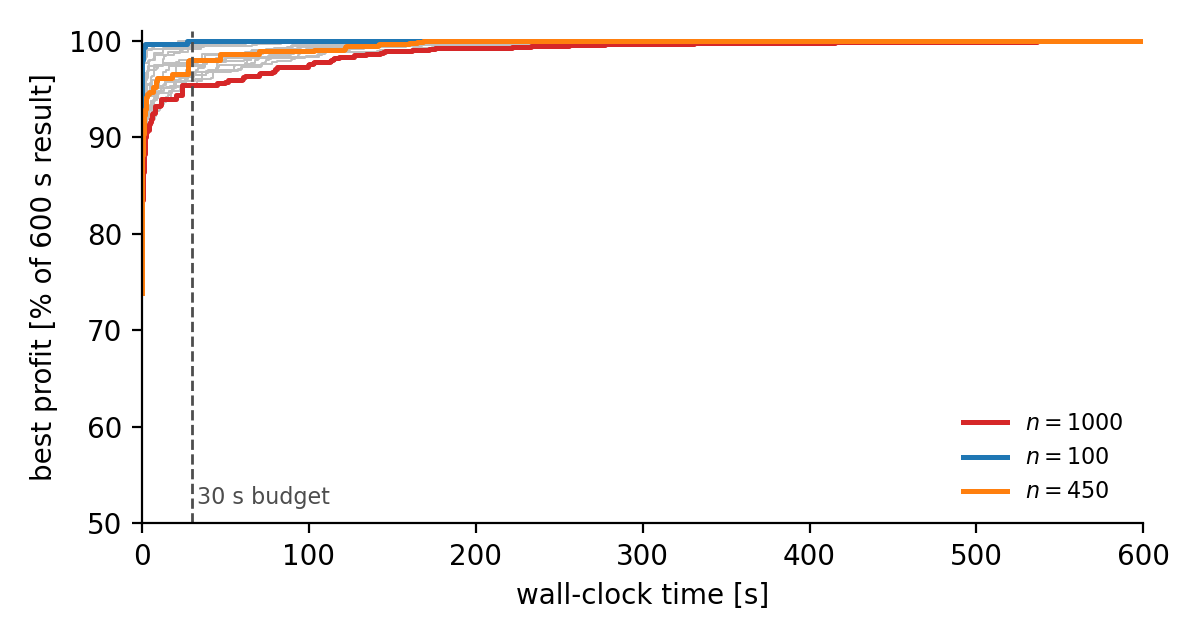
\includegraphics[width=0.85\linewidth]{convergence.png}
\caption{Best-solution convergence over 600\,s. The $y$-axis shows the
best feasible profit found so far as a percentage of the same run's final
600\,s value, so every curve ends at 100\,\% and curves of differently
sized instances become comparable. Gray = all 20 instances, highlighted =
$n=100/450/1000$. The dashed line marks the official 30\,s budget, which
captures on average 97.8\,\% of the 600\,s quality.}
\label{fig:convergence}
\end{figure}

% -------------------------------------------------------------------------
\section{Conclusion}

We presented an ALNS for the prize-collecting Skill VRP that serves an
average of 63.3\,\% of the singleton upper bound across all 20 benchmark
instances within the official 30\,s budget, with feasibility verified by the
provided checker on every instance. In retrospect the method choice of
Section~2 held up for exactly the reasons it was made: destroy/repair moves
handle customer \emph{selection} natively (every repair may grow the
served set), and one single parameterization transferred across a benchmark
whose iteration throughput varies by two orders of magnitude, confirmed by
the flat tuning plateau. What distinguishes our ALNS is not any single
operator but the combination of runtime-normalized adaptive weights and a
time-based cooling schedule: together they make the wall-clock budget
itself the controlling parameter of the search, so the same solver degrades
gracefully from 30{,}000 iterations on $n=50$ to 600 on $n=1000$. The
single-trajectory nature of ALNS also carried the engineering, as
anticipated in Section~3.5. Because only one solution is worked on at any
time, the route and move caches exist exactly once and amortize over every
candidate test, whereas a population-based method such as hybrid genetic
search~\cite{vidal2022} would have to replicate or recompute this state
for every individual, making the same caching investment considerably less
effective under our time budget.
The main lessons match the development path: (i) fix the yardstick first: the cheap singleton bound made every
later design decision measurable. (ii) throughput before operator
richness: constant-time insertion tests via time slacks and per-route caches
were worth more than any single operator. (iii) measure instead of
argue: the ablation showed that every operator contributes on average and
that the problem-specific skill-scarcity removal earns its place, while the
parameter study showed a flat plateau that made further tuning pointless.
Future work: slack-induced string removals~\cite{christiaens2020} as a more
disruptive destroy step for the budget-bound large instances, insertion
scoring that accounts for consumed shift time rather than pure travel delta,
and a set-covering post-optimization over the pool of routes collected during
the search.

% -------------------------------------------------------------------------
\begin{thebibliography}{99}
\bibitem{shaw1998} P.~Shaw.
Using constraint programming and local search methods to solve vehicle
routing problems. \emph{CP 1998}, LNCS 1520, 417--431, 1998.

\bibitem{ropke2006} S.~Ropke, D.~Pisinger.
An adaptive large neighborhood search heuristic for the pickup and delivery
problem with time windows. \emph{Transportation Science} 40(4):455--472, 2006.

\bibitem{pisinger2007} D.~Pisinger, S.~Ropke.
A general heuristic for vehicle routing problems.
\emph{Computers \& Operations Research} 34(8):2403--2435, 2007.

\bibitem{savelsbergh1992} M.~W.~P.~Savelsbergh.
The vehicle routing problem with time windows: minimizing route duration.
\emph{ORSA Journal on Computing} 4(2):146--154, 1992.

\bibitem{vansteenwegen2011} P.~Vansteenwegen, W.~Souffriau, D.~Van Oudheusden.
The orienteering problem: a survey.
\emph{European Journal of Operational Research} 209(1):1--10, 2011.

\bibitem{gunawan2016} A.~Gunawan, H.~C.~Lau, P.~Vansteenwegen.
Orienteering problem: a survey of recent variants, solution approaches and
applications. \emph{European Journal of Operational Research}
255(2):315--332, 2016.

\bibitem{labadie2012} N.~Labadie, R.~Mansini, J.~Melechovsk\'y,
R.~Wolfler Calvo. The team orienteering problem with time windows: an
LP-based granular variable neighborhood search.
\emph{European Journal of Operational Research} 220(1):15--27, 2012.

\bibitem{hulim2014} Q.~Hu, A.~Lim.
An iterative three-component heuristic for the team orienteering problem
with time windows. \emph{European Journal of Operational Research}
232(2):276--286, 2014.

\bibitem{cappanera2011} P.~Cappanera, L.~G\'omez-Real, M.~G.~Scutell\`a.
The skill vehicle routing problem. \emph{Network Optimization (INOC 2011)},
LNCS 6701, 354--364, 2011.

\bibitem{kovacs2012} A.~A.~Kovacs, S.~N.~Parragh, K.~F.~Doerner,
R.~F.~Hartl. Adaptive large neighborhood search for service technician
routing and scheduling problems. \emph{Journal of Scheduling}
15(5):579--600, 2012.

\bibitem{cisse2017} M.~Ciss\'e, S.~Yal\c{c}{\i}nda\u{g}, Y.~Kergosien,
E.~\c{S}ahin, C.~Lent\'e, A.~Matta. OR problems related to home health care:
a review of relevant routing and scheduling problems.
\emph{Operations Research for Health Care} 13--14:1--22, 2017.

\bibitem{demir2012} E.~Demir, T.~Bekta\c{s}, G.~Laporte.
An adaptive large neighborhood search heuristic for the pollution-routing
problem. \emph{European Journal of Operational Research} 223(2):346--359,
2012.

\bibitem{hammami2020} F.~Hammami, M.~Rekik, L.~C.~Coelho.
A hybrid adaptive large neighborhood search heuristic for the team
orienteering problem. \emph{Computers \& Operations Research} 123:105034,
2020.

\bibitem{christiaens2020} J.~Christiaens, G.~Vanden Berghe.
Slack induction by string removals for vehicle routing problems.
\emph{Transportation Science} 54(2):417--433, 2020.

\bibitem{vidal2022} T.~Vidal.
Hybrid genetic search for the CVRP: open-source implementation and SWAP*
neighborhood. \emph{Computers \& Operations Research} 140:105643, 2022.
\end{thebibliography}

% -------------------------------------------------------------------------
\appendix
\section*{Appendix: Pseudocode of the construction heuristic and all operators}

This appendix complements the prose descriptions of Sections~3.1, 3.3
and~3.4. Shared machinery is stated once (Algorithms~4 and~9), the
operators are then given as instantiations of the shared skeletons or as
individual algorithms. Throughout, $x$ is the current (partial) solution
and $\mathit{rand}()$ draws uniformly from $[0,1)$.

\subsection*{A.1\quad Construction heuristic}

\begin{center}
\begin{minipage}{0.92\linewidth}
\small
\hrule\vspace{2pt}
\textbf{Algorithm 3:} Greedy construction (also used, with shuffled order,
for restarts)
\vspace{2pt}\hrule\vspace{4pt}
\begin{tabbing}
\hspace{1.2em}\=\hspace{1.2em}\=\hspace{1.2em}\=\kill
$x \leftarrow$ empty plan (all couriers idle, all customers unserved)\\
$O \leftarrow$ customers with $\ge 1$ compatible courier, sorted by
decreasing profit $p_i$\\
\textbf{for} $i \in O$ \textbf{do}\\
\>$best \leftarrow \varnothing$\\
\>\textbf{for} courier $k$ with $Q_i \subseteq S_k$,
  position $j$ in route of $k$ \textbf{do}\\
\>\>\textbf{if} inserting $i$ at $(k, j)$ keeps time windows, shift and
  return time feasible\\
\>\>\textbf{and} travel-time increase $<$ that of $best$
  \textbf{then} $best \leftarrow (k, j)$\\
\>\textbf{if} $best \neq \varnothing$ \textbf{then} insert $i$ at $best$
  \quad\emph{(else leave $i$ unserved)}\\
\textbf{return} $x$
\end{tabbing}
\vspace{2pt}\hrule
\end{minipage}
\end{center}

Every insertion is checked for feasibility before it is applied, so the
returned plan is feasible at every intermediate step. With no feasible
insertion at all, the empty (feasible) plan is returned. The randomized
variant used for restarts (Section~3.2) replaces the profit ordering by a
uniformly shuffled order and is otherwise identical.

\subsection*{A.2\quad Shared destroy machinery}

All destroy operators determine their removal size the same way and share
a biased selection primitive.

\begin{center}
\begin{minipage}{0.92\linewidth}
\small
\hrule\vspace{2pt}
\textbf{Algorithm 4:} Shared destroy helpers
\vspace{2pt}\hrule\vspace{4pt}
\begin{tabbing}
\hspace{1.2em}\=\hspace{1.2em}\=\kill
\textbf{function} removalSize($x$):\\
\>$f \leftarrow$ uniform sample from the operator's fraction range
  $[f_{\min}, f_{\max}]$\\
\>\textbf{return} $q = \min\bigl(\max(1, \text{round}(f \cdot
  |\text{served}|)),\ \min(100, 0.25\,n),\ |\text{served}|\bigr)$\\[3pt]
\textbf{function} biasedPick(sorted pool $P$, bias $\beta$):
  \quad\emph{(worst / most related element first)}\\
\>\textbf{return and remove} $P[\lfloor \mathit{rand}()^{\beta}
  \cdot |P| \rfloor]$\\[3pt]
\textbf{function} finishDestroy(removed set $R$):\\
\>remove every $c \in R$ from its route, mark unserved, record origin
  route and position\\
\>rebuild the route caches of all affected couriers\\
\>\textbf{return} partial solution and $R$ as candidate pool for the repair
\end{tabbing}
\vspace{2pt}\hrule
\end{minipage}
\end{center}

$\beta > 1$ concentrates the picks near the front of the ranking without
making them deterministic (Shaw's randomization), so repeated calls do not
remove identical sets.

\subsection*{A.3\quad Ranking-based destroy operators}

Seven operators share one skeleton and differ only in the ranking
criterion.

\begin{center}
\begin{minipage}{0.92\linewidth}
\small
\hrule\vspace{2pt}
\textbf{Algorithm 5:} Ranking-based removal (skeleton)
\vspace{2pt}\hrule\vspace{4pt}
\begin{tabbing}
\hspace{1.2em}\=\hspace{1.2em}\=\kill
$q \leftarrow$ removalSize($x$),\quad
$P \leftarrow$ served customers sorted by criterion (worst first)\\
\textbf{repeat} $q$ times: $R \leftarrow R \cup{}$ biasedPick($P, \beta$)
\quad\emph{(random / worst-density / scarcity: plain top-$q$ cut)}\\
\textbf{return} finishDestroy($R$)
\end{tabbing}
\vspace{2pt}\hrule
\end{minipage}
\end{center}

\noindent Criteria (rank ascending, i.e.\ smallest value removed first):
\begin{itemize}\itemsep1pt
\item \emph{random removal}: no criterion, $R$ is a uniform sample of size
  $q$.
\item \emph{worst-density removal}: static profit density
  $p_c / (\text{minimal travel and service time of } c)$ plus additive
  noise $0.05 \cdot \mathit{rand}()$, top-$q$ cut.
\item \emph{skill-scarcity removal}: $p_c / (1 + d_{k(c)})$ where $k(c)$ is
  the courier of $c$ and $d_k$ counts unserved customers whose skills
  courier $k$ could serve. Low profit on a contested courier is removed
  first, top-$q$ cut.
\item \emph{worst-detour removal}: current-position profit per detour
  $p_c / (\max(\delta_c, 0) + 1)$ with
  $\delta_c = d(\mathit{prev}, c) + d(c, \mathit{next}) -
  d(\mathit{prev}, \mathit{next})$, biased picks with $\beta = 4$.
\item \emph{worst-detour removal v2}: same ratio multiplied by a noise
  factor in $[0.95, 1.05]$, biased picks with $\beta = 3$.
\item \emph{largest-saving removal}: detour $\delta_c$ alone, largest
  first, profit deliberately ignored, biased picks with $\beta = 3$.
\item \emph{history-based removal}: gap $\delta_c -
  \delta_c^{\text{best}}$, where $\delta_c^{\text{best}}$ is the smallest
  detour ever observed for $c$ in this run (updated on every call),
  largest gap first, biased picks with $\beta = 3$.
\end{itemize}

\subsection*{A.4\quad Relatedness-based destroy operators}

Four operators grow a removal set from a random seed and differ only in
the relatedness measure $r(i,j)$ (smaller = more related).

\begin{center}
\begin{minipage}{0.92\linewidth}
\small
\hrule\vspace{2pt}
\textbf{Algorithm 6:} Seed-growth removal (skeleton)
\vspace{2pt}\hrule\vspace{4pt}
\begin{tabbing}
\hspace{1.2em}\=\hspace{1.2em}\=\kill
$q \leftarrow$ removalSize($x$),\quad
$R \leftarrow \{\text{random served seed}\}$\\
\textbf{while} $|R| < q$ \textbf{do}\\
\>$s \leftarrow$ random element of $R$\\
\>$P \leftarrow$ up to 100 nearest still-served neighbors of $s$, sorted
  by $r(s, \cdot)$\\
\>$R \leftarrow R \cup{}$ biasedPick($P,\ \beta{=}4$)\\
\textbf{return} finishDestroy($R$)
\end{tabbing}
\vspace{2pt}\hrule
\end{minipage}
\end{center}

\noindent Relatedness measures ($\hat d$ = distance normalized by the
maximum distance, $\hat t$ = time difference normalized by the planning
horizon, $J$ = Jaccard similarity of required skill sets):
\begin{itemize}\itemsep1pt
\item \emph{related removal}: $r = \hat d(i,j)$ only (neighbor list is
  pre-sorted by distance, no re-sorting needed).
\item \emph{Shaw removal}: $r = 0.5\,\hat d + 0.25\,\hat t_{\text{ready}}
  + 0.25\,(1 - J)$ on the static ready times.
\item \emph{time-only Shaw removal}: $r = \hat t_{\text{ready}}$, distance
  and skills ignored.
\item \emph{temporal Shaw removal}: $r = 0.5\,\hat d +
  0.25\,\hat t_{\text{service}} + 0.25\,(1 - J)$, where
  $\hat t_{\text{service}}$ compares the \emph{current} service-begin
  times from the route caches.
\end{itemize}

\subsection*{A.5\quad Structural destroy operators}

\begin{center}
\begin{minipage}{0.92\linewidth}
\small
\hrule\vspace{2pt}
\textbf{Algorithm 7:} Route, sequence and time-window segment removal
\vspace{2pt}\hrule\vspace{4pt}
\begin{tabbing}
\hspace{1.2em}\=\hspace{1.2em}\=\kill
\emph{route removal:}\\
\>$P \leftarrow$ non-empty routes sorted by profit per used shift time
  (worst first)\\
\>\textbf{repeat} $1$ to $2$ times: empty the route biasedPick($P,\
  \beta{=}3$), add its customers to $R$\\[3pt]
\emph{sequence removal:}\\
\>$q \leftarrow$ removalSize($x$)\\
\>\textbf{for} routes in random order, until $|R| = q$: add a random
  contiguous segment of the route\\[3pt]
\emph{time-window segment removal:}\\
\>pick a random served customer, center a window of width
  $0.15 \cdot \text{horizon}$ at its service start\\
\>$R \leftarrow$ all customers whose cached service start falls inside the
  window\\
\>\textbf{if} $|R| > q_{\max}$ \textbf{then} $R \leftarrow$ uniform sample
  of size $q_{\max}$\\[3pt]
\textbf{return} finishDestroy($R$) \quad\emph{(each variant)}
\end{tabbing}
\vspace{2pt}\hrule
\end{minipage}
\end{center}

\begin{center}
\begin{minipage}{0.92\linewidth}
\small
\hrule\vspace{2pt}
\textbf{Algorithm 8:} Cluster removal (Kovacs et al.\ 2012)
\vspace{2pt}\hrule\vspace{4pt}
\begin{tabbing}
\hspace{1.2em}\=\hspace{1.2em}\=\kill
$q \leftarrow$ removalSize($x$),\quad
$v \leftarrow$ random route with $\ge 3$ customers
\quad\emph{(none: uniform sample, done)}\\
\textbf{while} $|R| < q$ \textbf{do}\\
\>build the minimum spanning tree over the remaining customers of $v$,
  drop its longest edge\\
\>add one of the two resulting clusters (coin flip) to $R$\\
\>$v \leftarrow$ route of the nearest still-served neighbor of a random
  removed customer\\
\>\textbf{if} no such splittable route exists \textbf{then break}\\
\textbf{return} finishDestroy($R$)
\end{tabbing}
\vspace{2pt}\hrule
\end{minipage}
\end{center}

\subsection*{A.6\quad Shared repair machinery}

\begin{center}
\begin{minipage}{0.92\linewidth}
\small
\hrule\vspace{2pt}
\textbf{Algorithm 9:} Shared repair helpers
\vspace{2pt}\hrule\vspace{4pt}
\begin{tabbing}
\hspace{1.2em}\=\hspace{1.2em}\=\kill
\textbf{function} candidatePool(removed $R$):\\
\>$C \leftarrow R$ (still unserved) $\cup$ up to 40 extra unserved
  customers,\\
\>\quad half of them the best by static profit density, half a uniform
  sample\\
\>\textbf{return} $C$\\[3pt]
\textbf{function} best($c$): \quad\emph{(uses the cached time slacks of
  Section~3.5)}\\
\>over all compatible couriers $k$ and positions $j$: evaluate
  $\Delta(c,k,j) = p_c - \text{penalty increase}$\\
\>\textbf{return} the move maximizing $\Delta$, ties broken by smaller
  travel delta\\[3pt]
\textbf{function} applyMove($m$): insert, rebuild the cache of the changed
route, rescan only that courier
\end{tabbing}
\vspace{2pt}\hrule
\end{minipage}
\end{center}

\subsection*{A.7\quad Best-first repairs}

Four repairs re-evaluate all candidates before every insertion and differ
in the selection rule.

\begin{center}
\begin{minipage}{0.92\linewidth}
\small
\hrule\vspace{2pt}
\textbf{Algorithm 10:} Best-first repair (skeleton)
\vspace{2pt}\hrule\vspace{4pt}
\begin{tabbing}
\hspace{1.2em}\=\hspace{1.2em}\=\kill
$C \leftarrow$ candidatePool($R$)\\
\textbf{loop}\\
\>\textbf{for} $c \in C$ with best($c$) $\neq \varnothing$ and
  $\Delta > 0$: compute the selection key of $c$\\
\>\textbf{if} no such $c$ \textbf{then break}\\
\>applyMove(best move of the $c$ with the best key),\quad
  $C \leftarrow C \setminus \{c\}$\\
\textbf{return} repaired solution
\end{tabbing}
\vspace{2pt}\hrule
\end{minipage}
\end{center}

\noindent Selection keys:
\begin{itemize}\itemsep1pt
\item \emph{greedy best insertion}: largest $\Delta$.
\item \emph{noisy greedy insertion}: largest $\Delta / (1 +
  \max(0, \text{travel delta}))$ times a noise factor in $[0.85, 1.15]$
  (the applied move itself is evaluated exactly).
\item \emph{regret-2 insertion}: largest $\Delta_1 - \Delta_2$ over the
  two best \emph{positions}, customers with a single feasible position
  get an urgency bonus.
\item \emph{regret-3 courier insertion}: largest
  $\sum_{i=2}^{3}(\text{travel}_i - \text{travel}_1)$ over the best
  insertions on three \emph{distinct couriers}, plus a large urgency bonus
  per missing courier alternative.
\end{itemize}

\subsection*{A.8\quad Single-pass repairs}

Five repairs visit each candidate exactly once, in an operator-specific
order, and insert it at its best (or a random) feasible position.

\begin{center}
\begin{minipage}{0.92\linewidth}
\small
\hrule\vspace{2pt}
\textbf{Algorithm 11:} Single-pass repair (skeleton)
\vspace{2pt}\hrule\vspace{4pt}
\begin{tabbing}
\hspace{1.2em}\=\hspace{1.2em}\=\kill
$C \leftarrow$ candidatePool($R$), ordered by the operator rule\\
\textbf{for} $c \in C$ \textbf{do}\\
\>$m \leftarrow$ best($c$)
  \quad\emph{(random-position: uniform choice among all feasible
  positions)}\\
\>\textbf{if} $m \neq \varnothing$ and $\Delta(m) > 0$ \textbf{then}
  applyMove($m$)\\
\textbf{return} repaired solution
\end{tabbing}
\vspace{2pt}\hrule
\end{minipage}
\end{center}

\noindent Orderings:
\begin{itemize}\itemsep1pt
\item \emph{sequential cheapest insertion}: decreasing profit, ties by
  tighter time window.
\item \emph{scarce-skill-first insertion}: increasing number of compatible
  couriers, then decreasing profit and profit density.
\item \emph{last-removed-first-inserted}: reverse removal order, extra
  candidates afterwards.
\item \emph{random-position insertion}: uniformly shuffled order, each
  customer at a uniformly random feasible position (pure
  diversification).
\item \emph{Shaw insertion}: first customer random, afterwards always the
  candidate most related (Shaw measure of A.4) to the last inserted one,
  picked with bias $\beta = 4$.
\end{itemize}

\end{document}
